
\documentclass{article}
\usepackage{tikz, amsmath, amssymb, graphicx, subcaption, listings,xcolor,makeidx}  % For \mathbb command
\usetikzlibrary{automata,positioning}
\makeindex


\definecolor{codegreen}{rgb}{0,0.6,0}
\definecolor{codegray}{rgb}{0.5,0.5,0.5}
\definecolor{codepurple}{rgb}{0.58,0,0.82}
\definecolor{backcolour}{rgb}{0.95,0.95,0.92}

\lstdefinestyle{mystyle}{
    backgroundcolor=\color{backcolour},   
    commentstyle=\color{codegreen},
    keywordstyle=\color{magenta},
    numberstyle=\tiny\color{codegray},
    stringstyle=\color{codepurple},
    basicstyle=\ttfamily\footnotesize,
    breakatwhitespace=false,         
    breaklines=true,                 
    captionpos=b,                    
    keepspaces=true,                 
    numbers=left,                    
    numbersep=5pt,                  
    showspaces=false,                
    showstringspaces=false,
    showtabs=false,                  
    tabsize=2
}

\renewcommand{\contentsname}{Índice}  % Cambia el nombre del índice

\lstset{style=mystyle}


    \title{Practicas MC}
    \date{\today}
    \author{Juan Luis Torres Ramos}


    \begin{document}
        
        % 
        % Portada
        % \pagenumbering{gobble}
        % \maketitle
        % \newpage
        % \pagenumbering{arabic}

        \begin{titlepage}
            \centering
            {
\includegraphics[width=1\textwidth]{./Imagenes/logo_universidad_de_granada.png}\par}
            \vspace{1cm}
            {\scshape\Large Escuela Tecnica Superior de Ingenieria Informatica y Telecomunicaciones \par}
            \vspace{2.5cm}
            {\scshape\Huge Practicas Modelos de Computación \par}
            \vspace{1cm}
            {\itshape\Large  Grupo B3 \par} 
            \vfill
            {\Large Juan Luis Torres Ramos \par}
            \vspace{0.5cm}
            {\large 15 Enero 2024 \par}
            \end{titlepage}
        
        \newpage  
        \tableofcontents
        \newpage 




        % introducción
        \section{Practica 1}
        Encuentra una gramática libre del contexto para generar cada uno de los siguientes lenguajes:

        \begin{enumerate}
            \item $L = \{a^i b^j \, | \, i, j \in \mathbb{N}, \, i \leq j\}$.
            \item $L = \{a^i b^j a^j b^i \, | \, i, j \in \mathbb{N}\}$.
            \item $L = \{a^i b^i a^j b^j \, | \, i, j \in \mathbb{N}\}$.
            \item $L = \{a_i b_i \,|\, i \in \mathbb{N}\} \cup \{b_i a_i \,|\, i \in \mathbb{N\}}$.
            \item $L = \{uu^{-1} \mid u \in \{a, b\}^*\}$.
            \item $L = \{a^i b^j c^{i+j} \, | \, i, j \in \mathbb{N}\}$.    
        \end{enumerate}

        \begin{flushleft}
            donde $\mathbb{N}$ es el conjunto de los numeros naturales incluyendo el 0
        \end{flushleft}

        \vspace{\baselineskip} % paso linea

        % Pasos que voy a seguir para resolver el ejercicio
        \begin{flushleft}
            
            \subsubsection*{Pasos para resolver el ejercicio:}
                        
            \begin{enumerate}
                \item Determinar los símbolos terminales y no terminales.
                \item Determinar el símbolo inicial.
                \item Analizar el lenguaje para determinar qué se pide.
                \item Determinar las reglas de producción.
                \item Comprobar con JFLAP  
            \end{enumerate}
        \end{flushleft}


        \newpage

        % 
        % APARTADO 1

        \subsection{$L = \{a^i b^j \, | \, i, j \in \mathbb{N}, \, i \leq j\}$.}

        \begin{flushleft}
            \begin{enumerate}
                \item Los símbolos terminales serán $\{a,b\}$ y los simbolos no terminales serán $S$ y $B$.
                \item El símbolo inicial será $S$.
                \item Analizar el lenguaje para determinar qué se pide. En este caso, se pide que la cadena tenga un número de $a$ menor o igual que el número de $b$. Por ejemplo, $aabbb$ y $aabb$ pertenecen al lenguaje, pero $aab$ no.
                \item Determino las reglas de producción:
                \begin{itemize}
                    \item $S \rightarrow \epsilon$ (genero la cadena vacía).
                    \item $S \rightarrow aSb$.
                    \item $S \rightarrow Sb$.
                \end{itemize}

                \item compruebo con JFLAP que la gramática es correcta.
                
                \vspace{\baselineskip} % paso linea

                % Imagenes en matriz
                \begin{figure}[h] 
                    \centering
                    \begin{subfigure}[b]{0.45\textwidth}
                        \centering
                        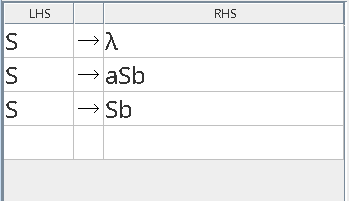
\includegraphics[width=\textwidth]{./Imagenes/produccion1.png}
                        \caption{la producción}
                        \label{fig:label1}
                    \end{subfigure}
                    \hfill
                    \begin{subfigure}[b]{0.45\textwidth}
                        \centering
                        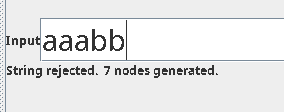
\includegraphics[width=\textwidth]{./Imagenes/grafoaaabb.png}
                        \caption{la cadena $aaabb$}
                        \label{fig:label2}
                    \end{subfigure}
                    \vspace{0.5cm} 
                    \\
                    \begin{subfigure}[b]{0.45\textwidth}
                        \centering
                        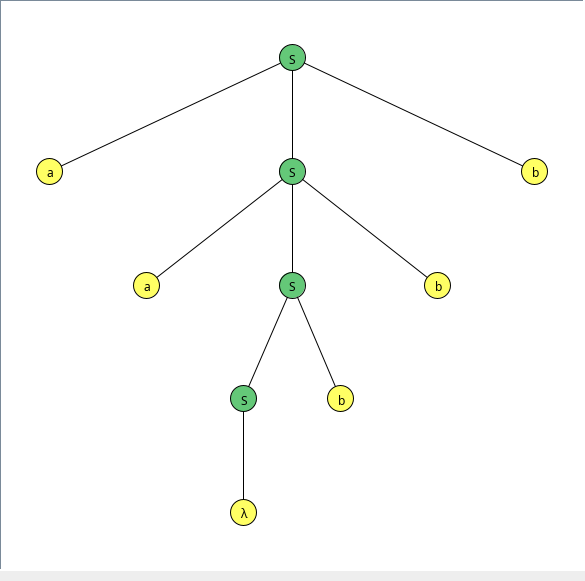
\includegraphics[width=\textwidth]{./Imagenes/grafoaabbb.png}
                        \caption{la cadena $aabbb$}
                        \label{fig:label3}
                    \end{subfigure}
                    \hfill
                    \begin{subfigure}[b]{0.45\textwidth}
                        \centering
                        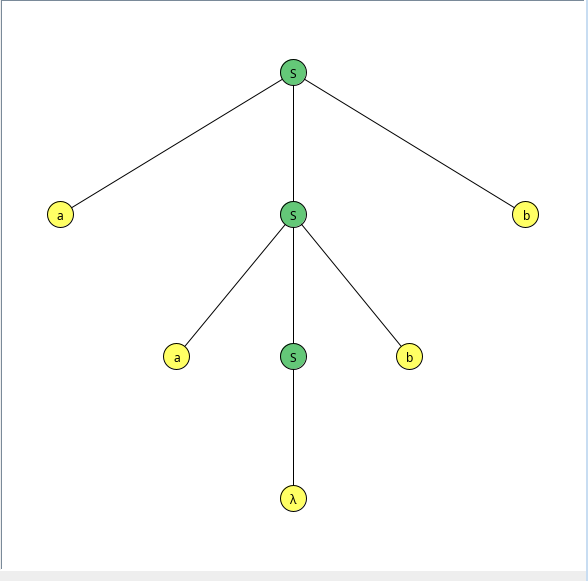
\includegraphics[width=\textwidth]{./Imagenes/grafoaabb.png}
                        \caption{la cadena $aabb$}
                        \label{fig:label4}
                    \end{subfigure}
                    \label{fig:matrix1}
                \end{figure}

                

                 

            \end{enumerate}
        \end{flushleft}

        % 
        % Apartado 2

        \newpage % paso pagina
        \subsection{$L = \{a^i b^j a^j b^i \, | \, i, j \in \mathbb{N}\}$.}
        \begin{flushleft}
            \begin{enumerate}

                \item Los símbolos terminales serán $\{a,b\}$ y los simbolos no terminales serán $S$ y $B$.

                \item El símbolo inicial será $S$.
            
                \item El lenguaje nos pide generar una cadena de 4 caracteres donde primero se generen $a^i b^j$ y luego $a^j b^i$, es decir en los extremos un numero caracteres $i$ y en los caracteres del centro un numero de caracteres $j$. 
                Por ejemplo, $aababb$ y $ab$ pertenecen al lenguaje, pero $aabbab$ no.

                \item Determino las reglas de producción:
                \begin{itemize}
                    \item $S \rightarrow aSb$ (genero mismo numero de caracteres en los extremos).
                    \item $S \rightarrow B$.
                    \item $B \rightarrow bBa$ (genero mismo numero de caracteres en el centro).
                    \item $B \rightarrow \epsilon$ (genero la cadena vacía).
                \end{itemize}

                \item compruebo con JFLAP que la gramática es correcta.

                % Imagenes en matriz
                \begin{figure}[h] 
                    \centering
                    \begin{subfigure}[b]{0.45\textwidth}
                        \centering
                        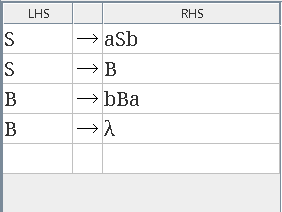
\includegraphics[width=\textwidth]{./Imagenes/produccion2.png}
                        \caption{la producción}
                        \label{fig:label5}
                    \end{subfigure}
                    \hfill
                    \begin{subfigure}[b]{0.45\textwidth}
                        \centering
                        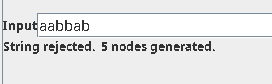
\includegraphics[width=\textwidth]{./Imagenes/grafo3.png}
                        \caption{la cadena $aabbab$}
                        \label{fig:label6}
                    \end{subfigure}
                    \vspace{0.5cm} 
                    \\
                    \begin{subfigure}[b]{0.45\textwidth}
                        \centering
                        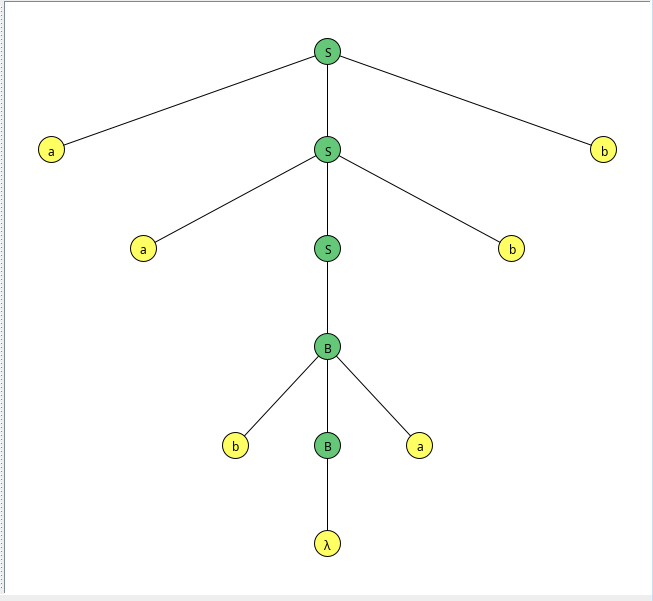
\includegraphics[width=\textwidth]{./Imagenes/grafo1.png}
                        \caption{la cadena $aababb$}
                        \label{fig:label7}
                    \end{subfigure}
                    \hfill
                    \begin{subfigure}[b]{0.45\textwidth}
                        \centering
                        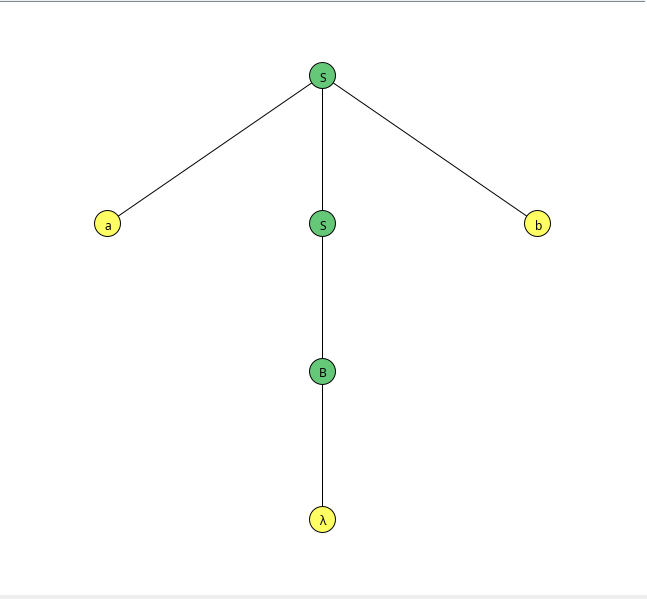
\includegraphics[width=\textwidth]{./Imagenes/grafo2.png}
                        \caption{la cadena $ab$}
                        \label{fig:label8}
                    \end{subfigure}
                    \label{fig:matrix2}
                \end{figure}

            \end{enumerate}
        \end{flushleft}
        
        
        % 
        % Apartado 3
        \newpage % paso pagina
        \subsection{$L = \{a^i b^i a^j b^j \, | \, i, j \in \mathbb{N}\}$.}
        \begin{flushleft}
            \begin{enumerate}
                \item Los símbolos terminales serán $\{a,b\}$ y los simbolos no terminales serán $S$ y $B$.
                \item El símbolo inicial será $S$.
                \item El lenguaje nos pide generar cadenas de 4 caracteres de la forma $abab$ donde los dos primeros caracteres tengan 
                el mismo numero de caracteres y para los dos ultimos caracteres tambien tengan la misma cantidad. Ejemplos de cadenas serían $aabbaabb$ ,$aabbab$ pero no acepta $aaba$
                \item Determino las reglas de producción:
                \begin{itemize}
                    \item $S \rightarrow AA$ (simbolo inicial).
                    \item $A \rightarrow aSb$. (genero $\{a^i b^i | i \in \mathbb{N}\}$).
                    \item $A \rightarrow \epsilon$ (genero la cadena vacía).
                \end{itemize}

                \item compruebo con JFLAP que la gramática es correcta.
                

                % Imagenes en matriz
                \begin{figure}[h] 
                    \centering
                    \begin{subfigure}[b]{0.45\textwidth}
                        \centering
                        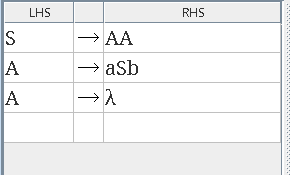
\includegraphics[width=\textwidth]{./Imagenes/produccion3.png}
                        \caption{la producción}
                        \label{fig:label10}
                    \end{subfigure}
                    \hfill
                    \begin{subfigure}[b]{0.45\textwidth}
                        \centering
                        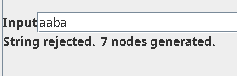
\includegraphics[width=\textwidth]{./Imagenes/grafo6.png}
                        \caption{la cadena $aaba$}
                        \label{fig:label11}
                    \end{subfigure}
                    \vspace{0.5cm} 
                    \\
                    \begin{subfigure}[b]{0.45\textwidth}
                        \centering
                        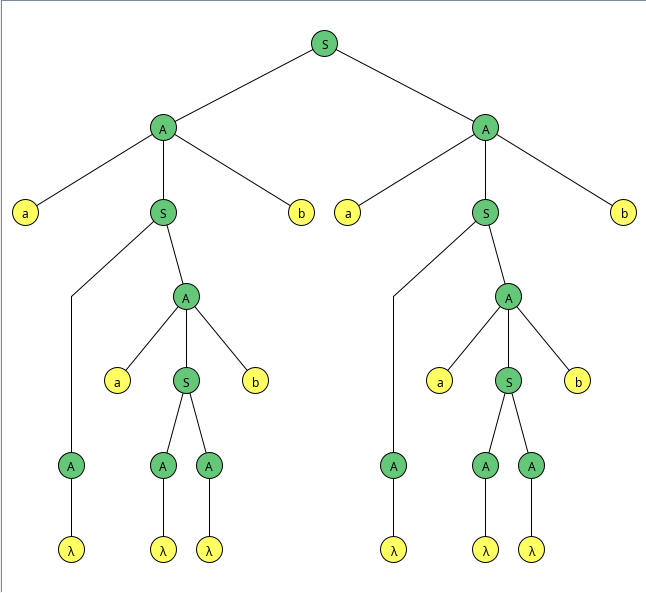
\includegraphics[width=\textwidth]{./Imagenes/grado4.png}
                        \caption{la cadena $aabbaabb$}
                        \label{fig:label12}
                    \end{subfigure}
                    \hfill
                    \begin{subfigure}[b]{0.45\textwidth}
                        \centering
                        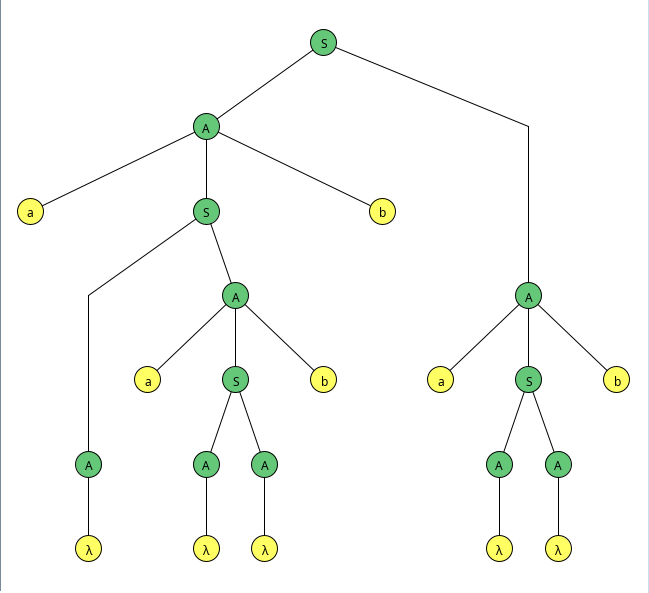
\includegraphics[width=\textwidth]{./Imagenes/grafo5.png}
                        \caption{la cadena $aabbab$}
                        \label{fig:label13}
                    \end{subfigure}
                    \label{fig:matrix3}
                \end{figure}

            \end{enumerate}
        \end{flushleft}



        % 
        % Apartado 4
        \newpage % paso pagina
        \subsection{$L = \{a_i b_i \,|\, i \in \mathbb{N}\} \cup \{b_i a_i \,|\, i \in \mathbb{N\}}$.}
        \begin{flushleft}
            \begin{enumerate}
                \item Los símbolos terminales serán $\{a,b\}$ y los simbolos no terminales serán $S$ , $A$ $B$.
                \item El símbolo inicial será $S$ .
                \item Combina dos conjuntos de cadenas: el primero contiene cadenas de la forma $\{a_i b_i \,|\, i \in \mathbb{N}\}$, y el segundo contiene cadenas de la forma $\{b_i a_i \,|\, i \in \mathbb{N}\}$.Las cadenas $aabb$ $bbaa$ lo cumplen mientras $abab$ no lo cumple Lo resolvemos por partes
                \item Determino las reglas de producción:
                
                \begin{itemize}
                    \item Podemos generar $\{a_i b_i \,|\, i \in \mathbb{N}\}. $
                        \subitem $A \rightarrow aAb$ , $A \rightarrow \epsilon$. 
                    \item Por otro lado $\{b_i a_i \,|\, i \in \mathbb{N}\}$.
                        \subitem $B \rightarrow bBa$ , $B \rightarrow \epsilon$ . 
                    \item El lenguaje L se puede generar añadiendo .
                        \subitem $S \rightarrow A$ , $S \rightarrow B$ . 
                \end{itemize}

                \item compruebo con JFLAP que la gramática es correcta.
                % Imagenes en matriz
                \begin{figure}[h] 
                    \centering
                    \begin{subfigure}[b]{0.25\textwidth}
                        \centering
                        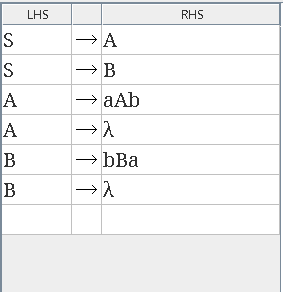
\includegraphics[width=\textwidth]{./Imagenes/produccion4.png}
                        \caption{la producción}
                        \label{fig:label14}
                    \end{subfigure}
                    \hfill
                    \begin{subfigure}[b]{0.4\textwidth}
                        \centering
                        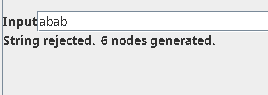
\includegraphics[width=\textwidth]{./Imagenes/grafoabab.png}
                        \caption{la cadena $abab$}
                        \label{fig:label15}
                    \end{subfigure}
                    \vspace{0.5cm} 
                    \\
                    \begin{subfigure}[b]{0.4\textwidth}
                        \centering
                        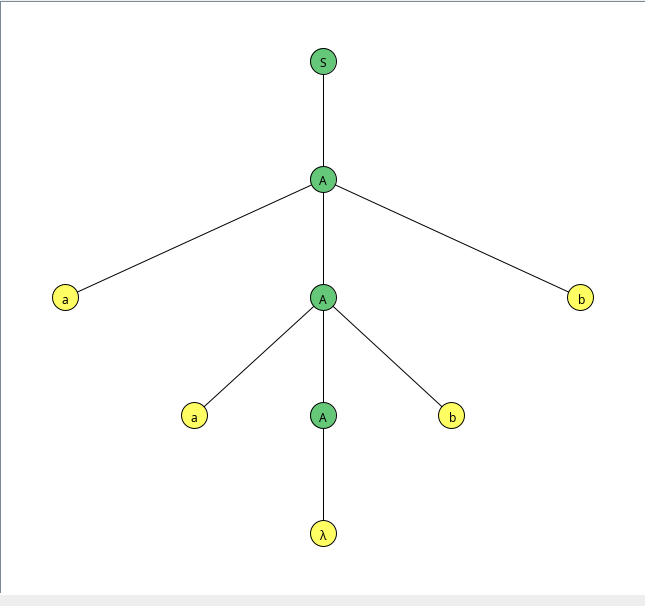
\includegraphics[width=\textwidth]{./Imagenes/grafo7.png}
                        \caption{la cadena $aabb$}
                        \label{fig:label16}
                    \end{subfigure}
                    \hfill
                    \begin{subfigure}[b]{0.4\textwidth}
                        \centering
                        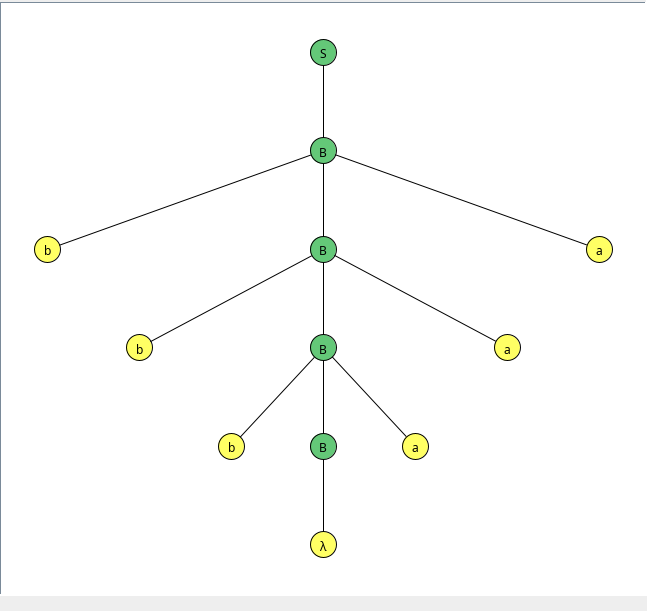
\includegraphics[width=\textwidth]{./Imagenes/grafobbbaaa.png}
                        \caption{la cadena $bbbaaa$}
                        \label{fig:label17}
                    \end{subfigure}
                    \label{fig:matrix4}
                \end{figure}



            \end{enumerate}
        \end{flushleft}
        % 
        % Apartado 5
        \newpage % paso pagina
        \subsection{$L = \{uu^{-1} \mid u \in \{a, b\}^*\}$.}
        \begin{flushleft}
            \begin{enumerate}
                \item Los símbolos terminales serán $\{a,b\}$ y los simbolos no terminales serán $S$.
                \item El símbolo inicial será $S$.
                \item Analizar el lenguaje para determinar qué se pide. En este caso,se pide generar 
                cadenas que son palíndromos formados por caracteres 'a' y 'b'. Cadenas que pertenecen al lenguaje son $abba$ y $bbaabb$ pero no $bbabb$. 
                \item Determino las reglas de producción:
                \begin{itemize}
                    \item $S \rightarrow \epsilon$ (genero la cadena vacía).
                    \item $S \rightarrow aSa$.
                    \item $S \rightarrow bSb$.
                \end{itemize}

                \item compruebo con JFLAP que la gramática es correcta.
                 % Imagenes en matriz
                 \begin{figure}[h] 
                    \centering
                    \begin{subfigure}[b]{0.45\textwidth}
                        \centering
                        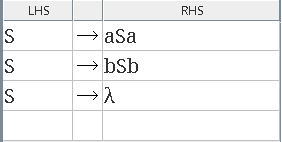
\includegraphics[width=\textwidth]{./Imagenes/produccion5.png}
                        \caption{la producción}
                        \label{fig:label18}
                    \end{subfigure}
                    \hfill
                    \begin{subfigure}[b]{0.45\textwidth}
                        \centering
                        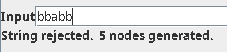
\includegraphics[width=\textwidth]{./Imagenes/grafo8.png}
                        \caption{la cadena $bbab$}
                        \label{fig:label19}
                    \end{subfigure}
                    \vspace{0.5cm} 
                    \\
                    \begin{subfigure}[b]{0.45\textwidth}
                        \centering
                        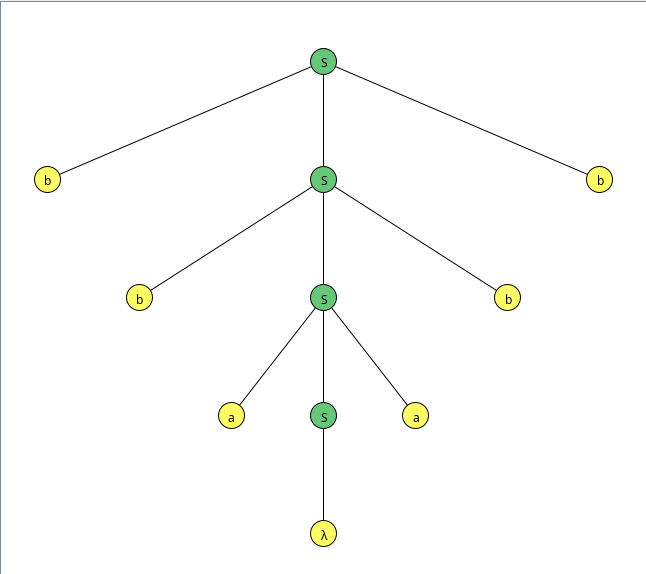
\includegraphics[width=\textwidth]{./Imagenes/grafo9.png}
                        \caption{la cadena $bbaabb$}
                        \label{fig:label20}
                    \end{subfigure}
                    \hfill
                    \begin{subfigure}[b]{0.45\textwidth}
                        \centering
                        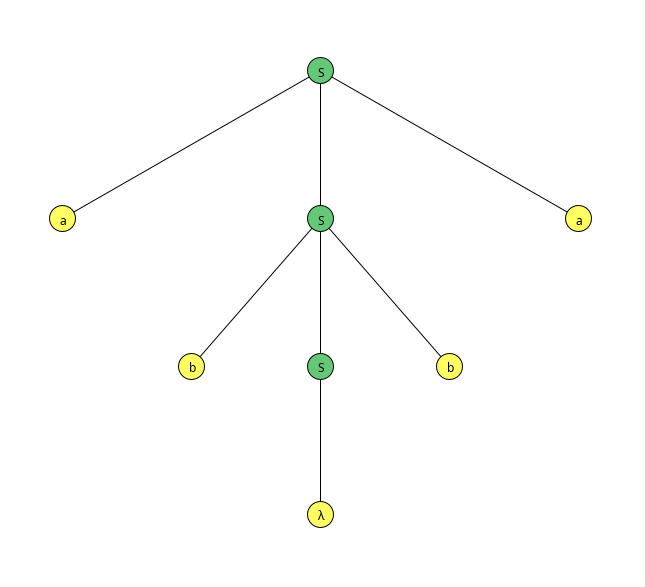
\includegraphics[width=\textwidth]{./Imagenes/grafo10.png}
                        \caption{la cadena $abba$}
                        \label{fig:label21}
                    \end{subfigure}
                    \label{fig:matrix5}
                \end{figure}

            \end{enumerate}
        \end{flushleft}

        % 
        % Apartado 6
        \newpage % paso pagina
        \subsection{$L = \{a^i b^j c^{i+j} \, | \, i, j \in \mathbb{N}\}$.}
        \begin{flushleft}
            \begin{enumerate}
                \item Los símbolos terminales serán $\{a,b,c\}$ y los simbolos no terminales serán $S$.
                \item El símbolo inicial será $S$.
                \item En este caso,se pide generar cadenas donde 
                la cantidad de 'a's y 'b's es igual y la cantidad total de 'c's es la suma de las cantidades de 'a' y 'b'
                . Cadenas que cumplen la gramatica son $abbccc$ y $aaabcccc$ pero no $bacc$
                \item Determino las reglas de producción:
                \begin{itemize}
                    \item $S \rightarrow aSc$ (genero la cadena vacía).
                    \item $S \rightarrow B$.
                    \item $B \rightarrow bBc$.
                    \item $B \rightarrow \epsilon$.
                \end{itemize}
                \item compruebo con JFLAP que la gramática es correcta.
                
                % Imagenes en matriz
                \begin{figure}[h] 
                    \centering
                    \begin{subfigure}[b]{0.45\textwidth}
                        \centering
                        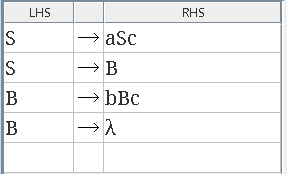
\includegraphics[width=\textwidth]{./Imagenes/produccion6.png}
                        \caption{la producción}
                        \label{fig:label22}
                    \end{subfigure}
                    \hfill
                    \begin{subfigure}[b]{0.45\textwidth}
                        \centering
                        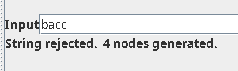
\includegraphics[width=\textwidth]{./Imagenes/grado11.png}
                        \caption{la cadena $bacc$}
                        \label{fig:label23}
                    \end{subfigure}
                    \vspace{0.5cm} 
                    \\
                    \begin{subfigure}[b]{0.45\textwidth}
                        \centering
                        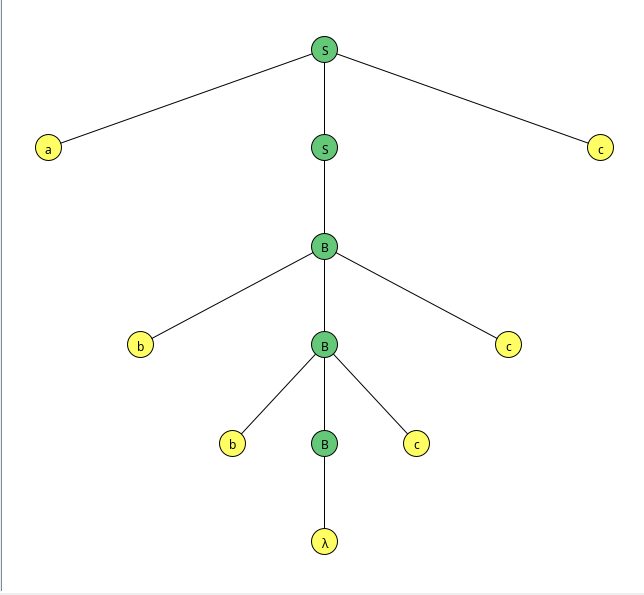
\includegraphics[width=\textwidth]{./Imagenes/grafo12.png}
                        \caption{la cadena $abbccc$}
                        \label{fig:label24}
                    \end{subfigure}
                    \hfill
                    \begin{subfigure}[b]{0.45\textwidth}
                        \centering
                        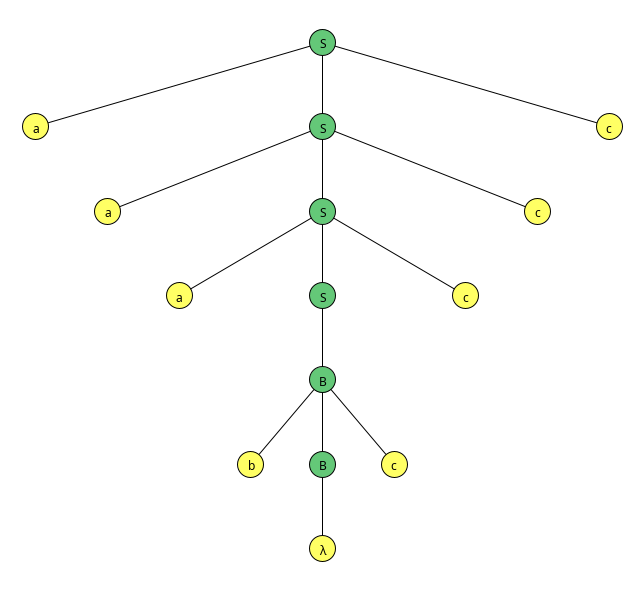
\includegraphics[width=\textwidth]{./Imagenes/grafo13.png}
                        \caption{la cadena $aaabcccc$}
                        \label{fig:label25}
                    \end{subfigure}
                    \label{fig:matrix6}
                \end{figure}


            \end{enumerate}
        \end{flushleft}


        \newpage


        %
        % PRACTICA 2
        \section{Practica 2}
        Analizadores léxicos, problemas de mineria, trabajo Lex.
        \subsection{Tareas a realizar}
        \begin{enumerate}
        \item Formar un grupo de trabajo compuesto por una, dos o tres personas.
        \item Cada grupo de trabajo debe pensar un problema original de procesamiento de textos. Para la resolución de este problema debe ser apropiado el uso de Lex, o sea, se debe resolver mediante el emparejamiento de cadenas con expresiones regulares y la asociación de acciones a cada emparejamiento.
        \item Cada grupo debe resolver el problema propuesto usando Lex. Se deberá realizar una memoria donde se presente una descripción del problema y su solución, además de entregar electrónicamente los ficheros de texto con la implementación de la solución.
        \item Esta práctica deberá ser entregada antes del día 15 de Enero de 2024. Se entregará a través de la plataforma PRADO en un fichero .zip conteniendo todos los archivos de esta práctica. Sólo es necesario que lo entregue uno de los componentes del grupo.
        \end{enumerate}

        \vspace{\baselineskip} % paso linea


        % Pasos que voy a seguir para resolver el ejercicio
        \begin{flushleft}
            
            \subsubsection*{Pasos para resolver el ejercicio:}
                        
            \begin{enumerate}
                \item Descripcion del problema 
                \item Solucion 
                \item Codigo lex
            \end{enumerate}
        \end{flushleft}

        \newpage

        \subsection{Descripcion del Problema}
        
        Soy un nuevo profesor de la asignatura de Fundamentos de Programacion. Tras corregir varios ejercicios de los alumnos me he dado cuenta que la cantidad de comentarios explicando 
        el codigo va relacionada con la nota del ejercicio. Por lo que he decidido crear un programa que calcule la densidad de comentarios en un codigo fuente en C para evaluar positivamente a los alumnos que comenten su codigo.
    
        \subsection{Densidad de comentarios codigo}
        Tu tarea es desarrollar un programa en Lex que calcule la densidad de comentarios en un código fuente en C. 
        La densidad de comentarios se define como el porcentaje del código total que está ocupado por comentarios. 

        \subsection{Pasos}
        El alumno ha entregado su ejercicio de C correspondiente de la asignatura, voy a calcular la densidad de comentarios con la siguiente formula: 
        \[ \text{{Densidad de comentarios}} = \frac{{\text{{Total de letras en un comentario}}}}{{\text{{Total de letras en el codigo}}}} \]
        
        \begin{enumerate}
            \item Creo 2 variables globales, para contar letras en el código y en comentarios.
            \item Defino 2 estados \texttt{INCOMMENTBLOCK} y \texttt{INCOMMENTLINE} para manejar por separado los dos tipos de comentarios en C: comentarios en línea y comentarios en bloque.
            \item Defino una función \texttt{contarLetras} que cuenta únicamente letras; no cuenta espacios en blanco, tabuladores, saltos de línea ni retornos de carro.
            \item Defino reglas de Flex para reconocer los comentarios:
                \begin{itemize}
                    \item Si encuentra ``/*'', comienza el subestado \texttt{INCOMMENTBLOCK} y termina con ``*/''.
                    \item Si encuentra ``//'', comienza el subestado \texttt{INCOMMENTLINE} y termina con un salto de línea.
                    \item Dentro del estado \texttt{INCOMMENTBLOCK}, selecciono para cualquier carácter que no sea un asterisco (para evitar contar el fin del comentario \texttt{*/}) ni un salto de línea. Para comentarios en línea, solo no cuento el salto de línea.
                    \item El texto seleccionado corresponde a la variable \texttt{yytext}, la cual introduzco en mi función \texttt{contarLetras}.
                    \item Imprimo cada comentario encontrado haciendo print a yytext, tambien indico tipo comentario y su longitud
                    \item Para referirme a todo el código, uso \texttt{.|\textbackslash n}, haciendo referencia a cualquier carácter y un salto de línea. Asi calculo la longitud total del fichero.

                \end{itemize}
            \item Por último, calculo la densidad de comentarios con la fórmula anterior.
        \end{enumerate}

        \vspace{\baselineskip} % paso linea

        Para ejecutar el programa usaremos un Makefile 

        \begin{lstlisting}[frame=single, caption={(a) Makefile}, captionpos=b, title=(a) Makefile]
    all: comentador

    comentador: lex.yy.c
        gcc -o comentador lex.yy.c -lfl
            
    lex.yy.c: comentador.l
        flex comentador.l
            
    run: comentador
        ./comentador < ./ejemplos/ejemplo1.c
        ./comentador < ./ejemplos/ejemplo2.c
\end{lstlisting}
    

    \begin{lstlisting}[frame=single, caption={Ejemplo de ejecución}, captionpos=b, title=(b) Ejemplo de ejecución]
    $ make all 
    $ make run 
\end{lstlisting}

            \vspace{\baselineskip} % paso linea
    
        \lstset{language=C, breaklines=true, basicstyle=\footnotesize}
        \begin{lstlisting}[frame=single, caption={Ejemplo1.c}, title= (c) Ejemplo1.c]       
    #include <stdio.h>
    #include <stdlib.h>
                
    // funcion de ejemplo
    void imprimirMensaje() {
        printf("! Hola, mundo!\n");
    }

    /*
        comentarios
        multilinea
    */

    int main{
        // Llamada a la funcion
        imprimirMensaje();
        return 0;
    }
\end{lstlisting}
\newpage
\begin{lstlisting}[frame=single, caption={Ejemplo2.c}, title=(d) Ejemplo2.c]  
    // Pepe1
    //  Pepe 1
    
    #include <stdio.h>
    #include <stdlib.h>
    
    void imprimirMensaje() // paso1: imprime mensaje en pantalla
    {
        printf("! Hola, mundo!\n");
    }
    
    /*
        ahora viene el main
    */
    
    
    int main // paso2: llamo a / la funcion
    {
        imprimirMensaje(); 
        return 0;
    }          
\end{lstlisting}


    \lstset{language=C, breaklines=true, basicstyle=\footnotesize}
        \begin{lstlisting}[frame=single, caption={Codigo Analizador Lex}, title=(e) Codigo Analizador Lex]        
    %{
    #include <stdio.h>
    #include <stdlib.h>
                
    int total_letters = 0;
    int comment_letters = 0;  
    int comment_letters_global = 0;         
    int contarLetras(const char* texto);         
    %}
                
    %x INCOMMENTBLOCK INCOMMENTLINE
                
    %%       
    "/*" {
        BEGIN(INCOMMENTBLOCK);
        printf("\nComentario en bloque: ");
        comment_letters = 0;
    }
                
    <INCOMMENTBLOCK>"*/" {
        BEGIN(INITIAL);
        printf("\nNumero de letras en comentario en bloque: %d\n", comment_letters);
        comment_letters = 0;
    }
                
    <INCOMMENTBLOCK>[^*\n]+ {
        int letras_comentario = contarLetras(yytext);
        printf("%s", yytext);
        comment_letters += letras_comentario;
        comment_letters_global += letras_comentario;
    }
                         
    <INCOMMENTBLOCK>\n {
        // No contar el salto de linea
    }
                
    "//" {
        BEGIN(INCOMMENTLINE);
        printf("\nComentario en linea: ");
    }
                
    <INCOMMENTLINE>\n {
        BEGIN(INITIAL);
        printf("\nNumero de letras en comentario en linea: %d\n", comment_letters);
        comment_letters = 0;
    }
                
    <INCOMMENTLINE>[^\n]+ {
        printf("%s", yytext);
        comment_letters += contarLetras(yytext);
        comment_letters_global += contarLetras(yytext);
    }
                
    .|\n {
        total_letters += contarLetras(yytext);
    }         
    %%     
    // sin salto de linea al final, solo cuento letras simbolos y numeros
    int contarLetras(const char* texto) {
        int contador = 0;
        while (*texto) {
            if (*texto != '\n' && *texto != '\t' && *texto != ' ' && *texto != '\r') {
                contador++;
                }
                texto++;
            }
        return contador;
    }       
    // conslato de linea
    int main(int argc, char* argv[]) {
        printf("DEBUG:\n");
        yylex();
                    
        printf("RESULTADO:\n");
        printf("\nNumero total de letras en codigo: %d\n", total_letters);
        printf("Numero total de letras en comentarios: %d\n", comment_letters_global );
        printf("Porcentaje de Comentarios: %.2f \%\n\n", (float)(comment_letters_global) / total_letters * 100);   
        return EXIT_SUCCESS;
    }
        \end{lstlisting}
    
        \newpage
        \begin{figure}[!h]
            \centering
            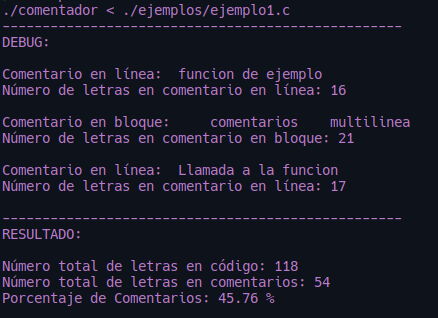
\includegraphics[width=0.8\textwidth]{./Imagenes/salida1.png}
            \caption*{(f) Resultado de la ejecución del programa}
        \end{figure}

        \begin{figure}[!h]
            \centering
            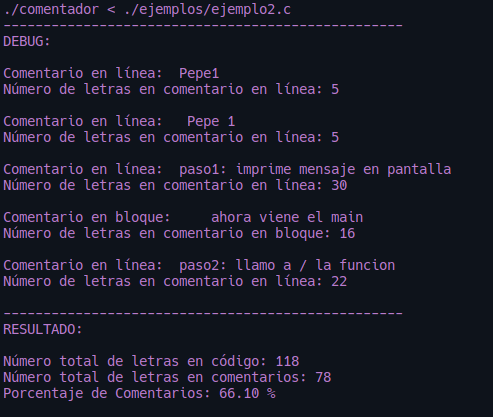
\includegraphics[width=0.8\textwidth]{./Imagenes/salida2.png}
            \caption*{(g) Resultado de la ejecución del programa}
        \end{figure}
        
        \subsubsection*{Analisis Resultado}
     Podemos ver que el programa ha detectado los comentarios y diferenciado si es un comentario en linea o 
     un comentario en bloque. Calcula correctamente tanto las letras de cada comentario como el total de letras en el codigo y por
     ultimo calcula el porcentaje de comentarios en el codigo  correspondiente.
     Ahora el maestro, viendo el porcentaje de comentarios de cada ejercicio de FP, puede evaluar positivamente a los alumnos que comenten su codigo correctamente.
     Tampoco se puede abusar de los comentarios, ya que el maestro puede ver el porcentaje de comentarios y si es demasiado alto puede penalizar al alumno.

    

    \newpage

    %
    % PRACTICA 3
    \section{Practica 3}
    Diseña una máquinas de estados finitos, en particular la máquina de Mealy, para simular la codificación y decodificación del código Enigma. Implementa un conjunto de estados y transiciones que reflejen el proceso de cifrado y descifrado característico del Enigma. Utiliza JFLAP para simular y visualizar la máquina de Mealy que actúa como codificador y decodificador.
    
    \vspace{\baselineskip} % paso linea
    \subsection{Maquina Enigma}
    Durante la Segunda Guerra Mundial, la máquina Enigma era utilizada para encifrar las comunicaciones militares de Alemania. La Enigma, creada por Arthur Scherbius y adoptada por el ejército alemán en los años 30, constaba de un teclado y rotores que se podían girar.    
    
    \vspace{\baselineskip} % paso linea
    Los rotores, que eran discos rotatorios con letras del alfabeto conectados eléctricamente en cascada, eran la fuente de la complejidad. Antes de cifrar un mensaje, se configuraban los rotores para determinar la sustitución de letras.

    \vspace{\baselineskip} % paso linea
    Un solo "reflector" reflejaba la señal a través de los rotores, lo que aumentaba la complejidad del cifrado. Además, después de cada pulsación, los rotores giraban, cambiando la configuración y dificultando los intentos de descifrado.

    
    \vspace{\baselineskip} % paso linea
    A pesar de la fuerza de la Enigma, los aliados, especialmente aquellos en Bletchley Park, lograron descifrar las comunicaciones encriptadas, lo que ayudó a las fuerzas del Eje a ganar.
    

    \begin{figure}[!h]
        \centering
        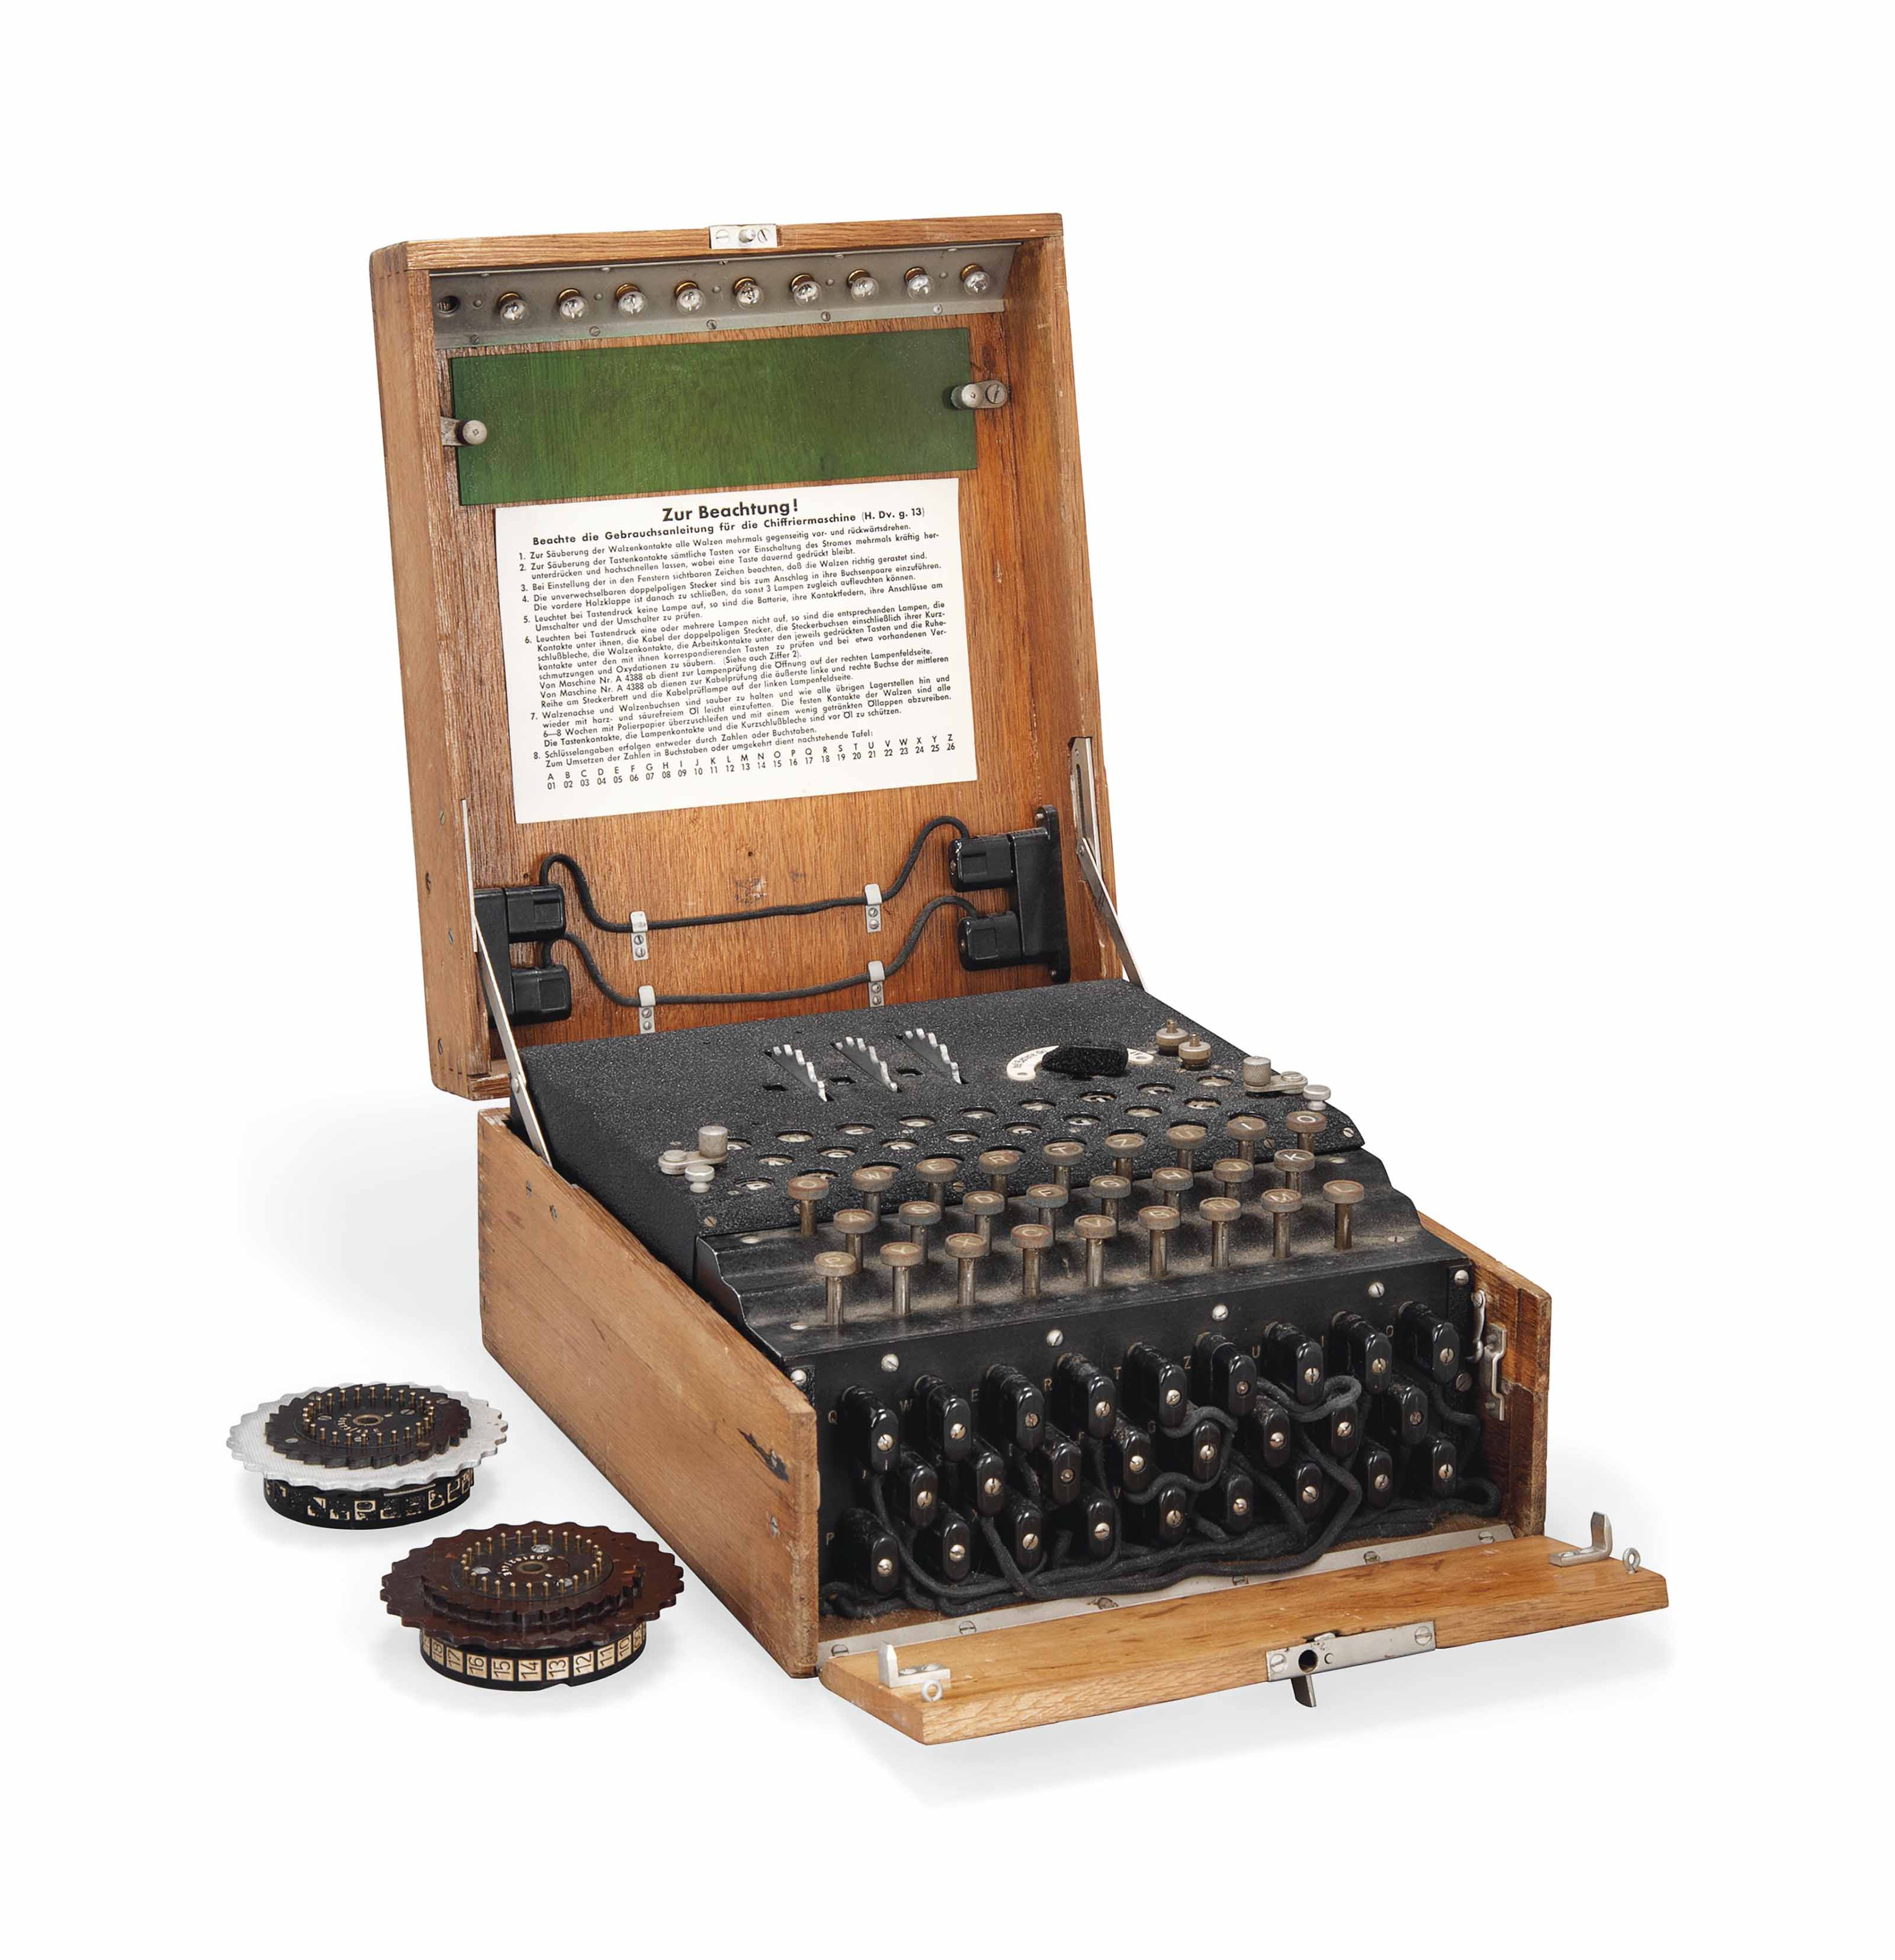
\includegraphics[width=0.5\textwidth]{./Imagenes/maquinaEnigma.jpg}
        \caption*{(a) Maquina Enigma}
    \end{figure}
    
    \newpage

    \subsection{Reglas}
    Debido a la complejidad de la máquina Enigma, he decidido mostrar las reglas básicas de reemplazo de letras en uno de sus rotores. Utilizo las entradas binarias 0 y 1 y sus respectivas salidas para mapear el rotor en mi representación.

    \vspace{\baselineskip} % paso linea

    Cada uno de los tres nodos de estado en el diagrama se llama A, B y C, y representa una configuración particular del rotor. Estos estados podrían referirse a las primeras ubicaciones de los rotores de la máquina Enigma.
    \vspace{\baselineskip} % paso linea

    Cada transición se representa con una flecha. Por ejemplo, una flecha de A a B está marcada con "0/1", lo que significa que si la entrada es 0, la salida será 1.
    \vspace{\baselineskip} % paso linea

    Reglas que he definido:
    \begin{itemize}
        \item De A a B: "1 / 1"
        \item De A a B: "1 / 0"
        \item De B a C: "0 / 1"
        \item De B a A: "1 / 0"
        \item De C a C: "1 / 0"
        \item De C a B: "0 / 1"
    \end{itemize}


    \newpage
    \subsection{Codificador}
    \begin{itemize}
        \item Entrada Binaria (0 o 1): Recibe una entrada binaria, por ejemplo, '01000101'.
        \item Transición a través de los Rotores: Aplica las reglas de sustitución del rotor correspondiente. Siguiendo el ejemplo, podría cambiar '10' a '11' según las reglas definidas.
        \item Salida Cifrada: La salida es la representación cifrada de la entrada original. En nuestro ejemplo, la salida sería '10111010'.
    \end{itemize}
    
    \vspace{\baselineskip} % paso linea
    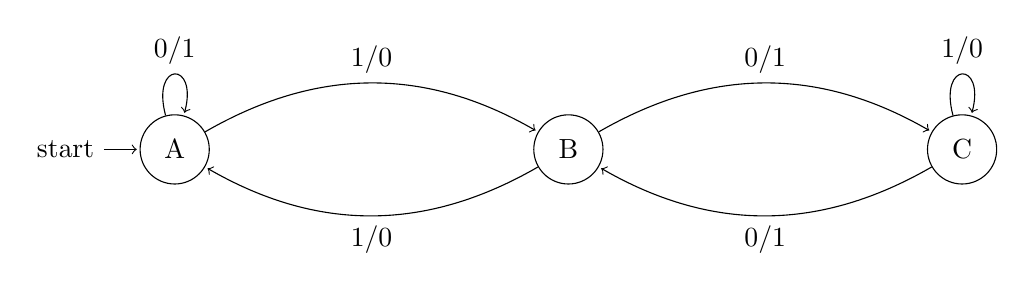
\begin{tikzpicture}[shorten >=1pt, node distance=5cm, on grid, auto]
        \node[state, initial] (A) {A};
        \node[state, right=of A] (B) {B};
        \node[state, right=of B] (C) {C};
      
        \path[->]
        (A) edge[bend left] node {1/0} (B)
            edge[loop above] node {0/1} ()
        (B) edge[bend left] node {0/1} (C)
            edge[bend left] node {1/0} (A)
        (C) edge[loop above] node {1/0} ()
            edge[bend left] node {0/1} (B);
    \end{tikzpicture}
    \vspace{\baselineskip} % paso linea
    \vspace{\baselineskip} % paso linea

    \begin{figure}[!h]
        \centering
        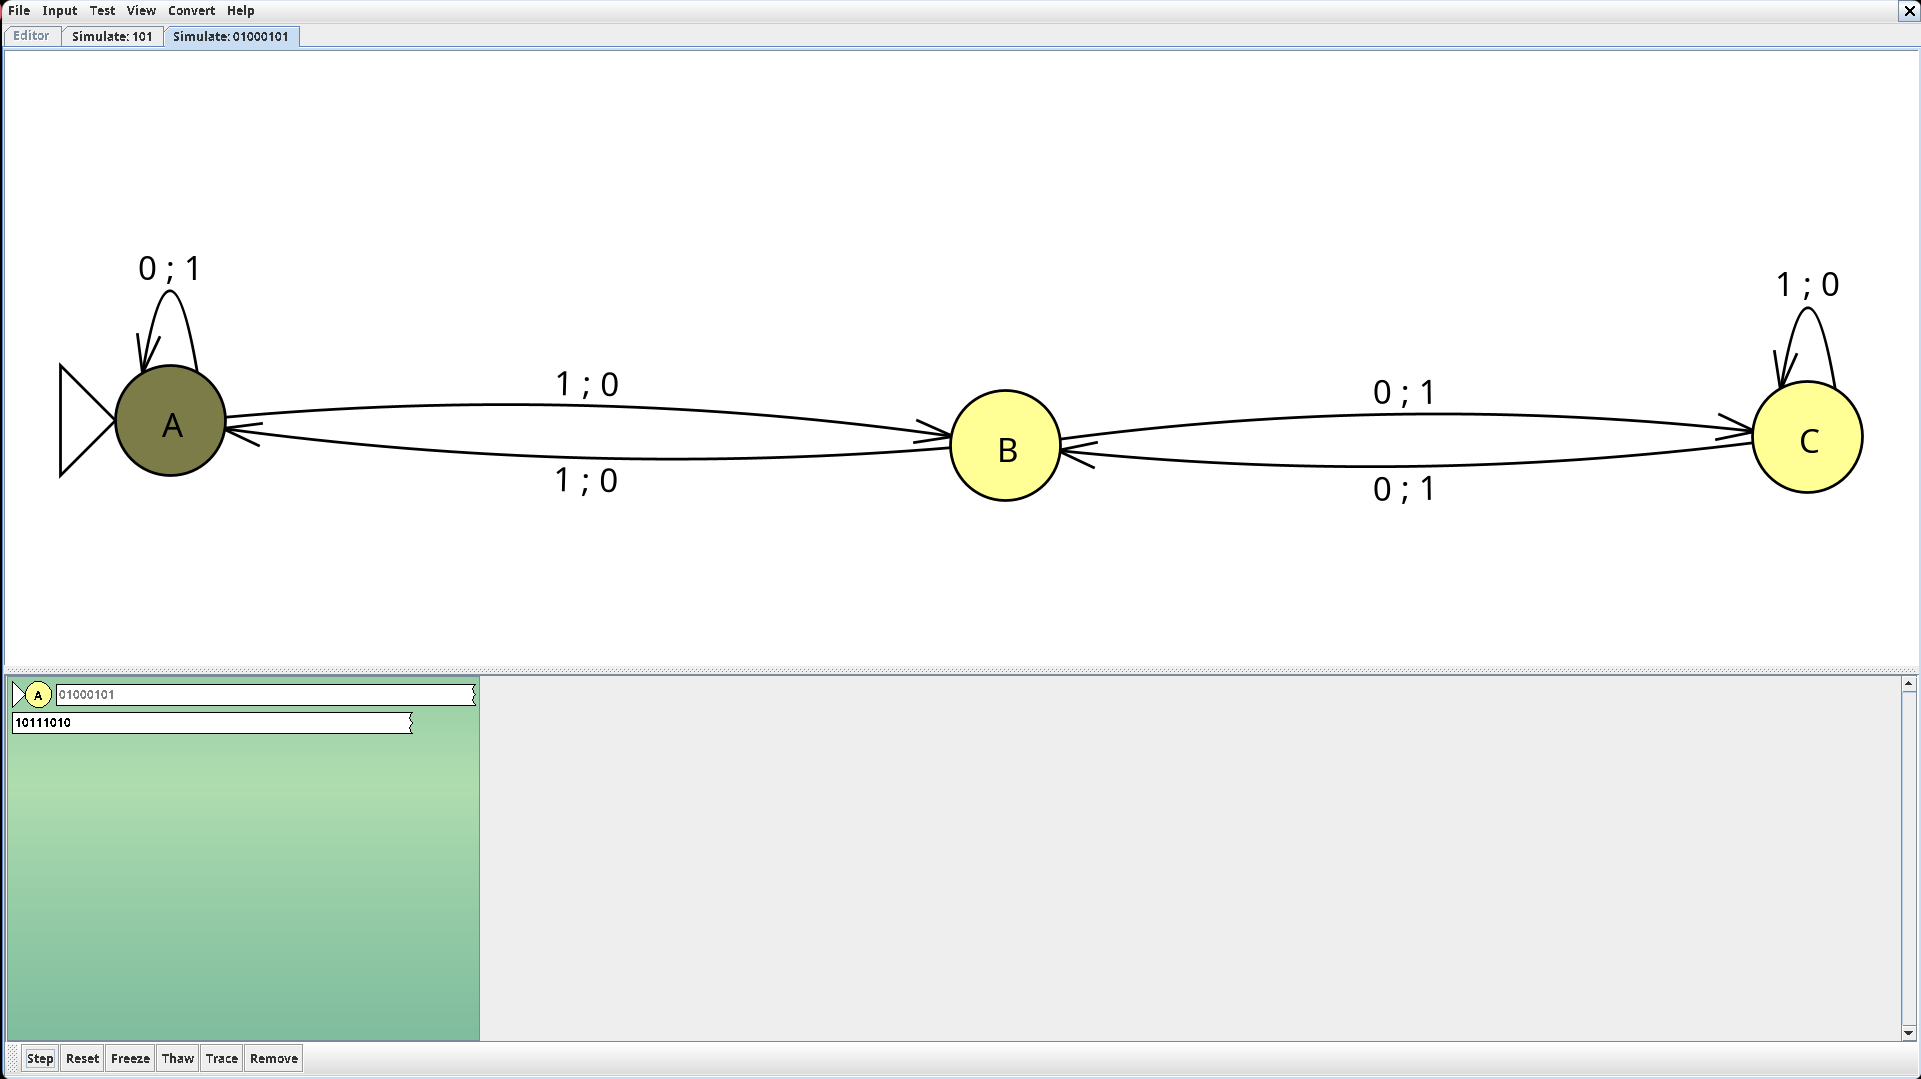
\includegraphics[width=1\textwidth]{./Imagenes/codificador.png}
        \caption*{(b) codificador}
    \end{figure}

    
    \newpage



    \subsection{Decodificador}
    Un decodificador es, en esencia, una máquina de estados finitos que hace lo que un codificador hace. El codificador de tu caso tenía entradas y salidas, y el decodificador debe tener entradas y salidas para revertir ese proceso.    

    \begin{itemize}
        \item Entrada Binaria (0 o 1): Recibe la entrada binaria de salida del codificador, por ejemplo, '10111010'.
        \item Transición a través de los Rotores: Aplica las reglas de sustitución del rotor correspondiente, pero esta vez a la inversa.
        \item Salida Cifrada: La salida es la salida original luego de cifrarlo. En nuestro ejemplo, la salida sería '01000101'.
    \end{itemize}

    \vspace{\baselineskip} % paso linea
    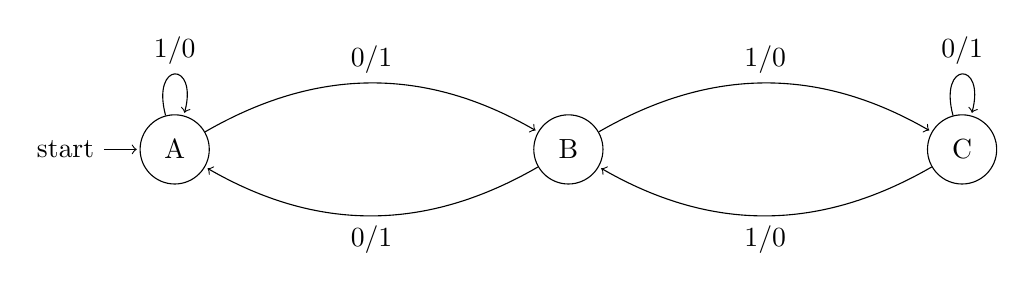
\begin{tikzpicture}[shorten >=1pt, node distance=5cm, on grid, auto]
        \node[state, initial] (A) {A};
        \node[state, right=of A] (B) {B};
        \node[state, right=of B] (C) {C};
      
        \path[->]
        (A) edge[bend left] node {0/1} (B)
            edge[loop above] node {1/0} ()
        (B) edge[bend left] node {1/0} (C)
            edge[bend left] node {0/1} (A)
        (C) edge[loop above] node {0/1} ()
            edge[bend left] node {1/0} (B);
    \end{tikzpicture}
    
    \vspace{\baselineskip} % paso linea
    \vspace{\baselineskip} % paso linea

    \begin{figure}[!h]
        \centering
        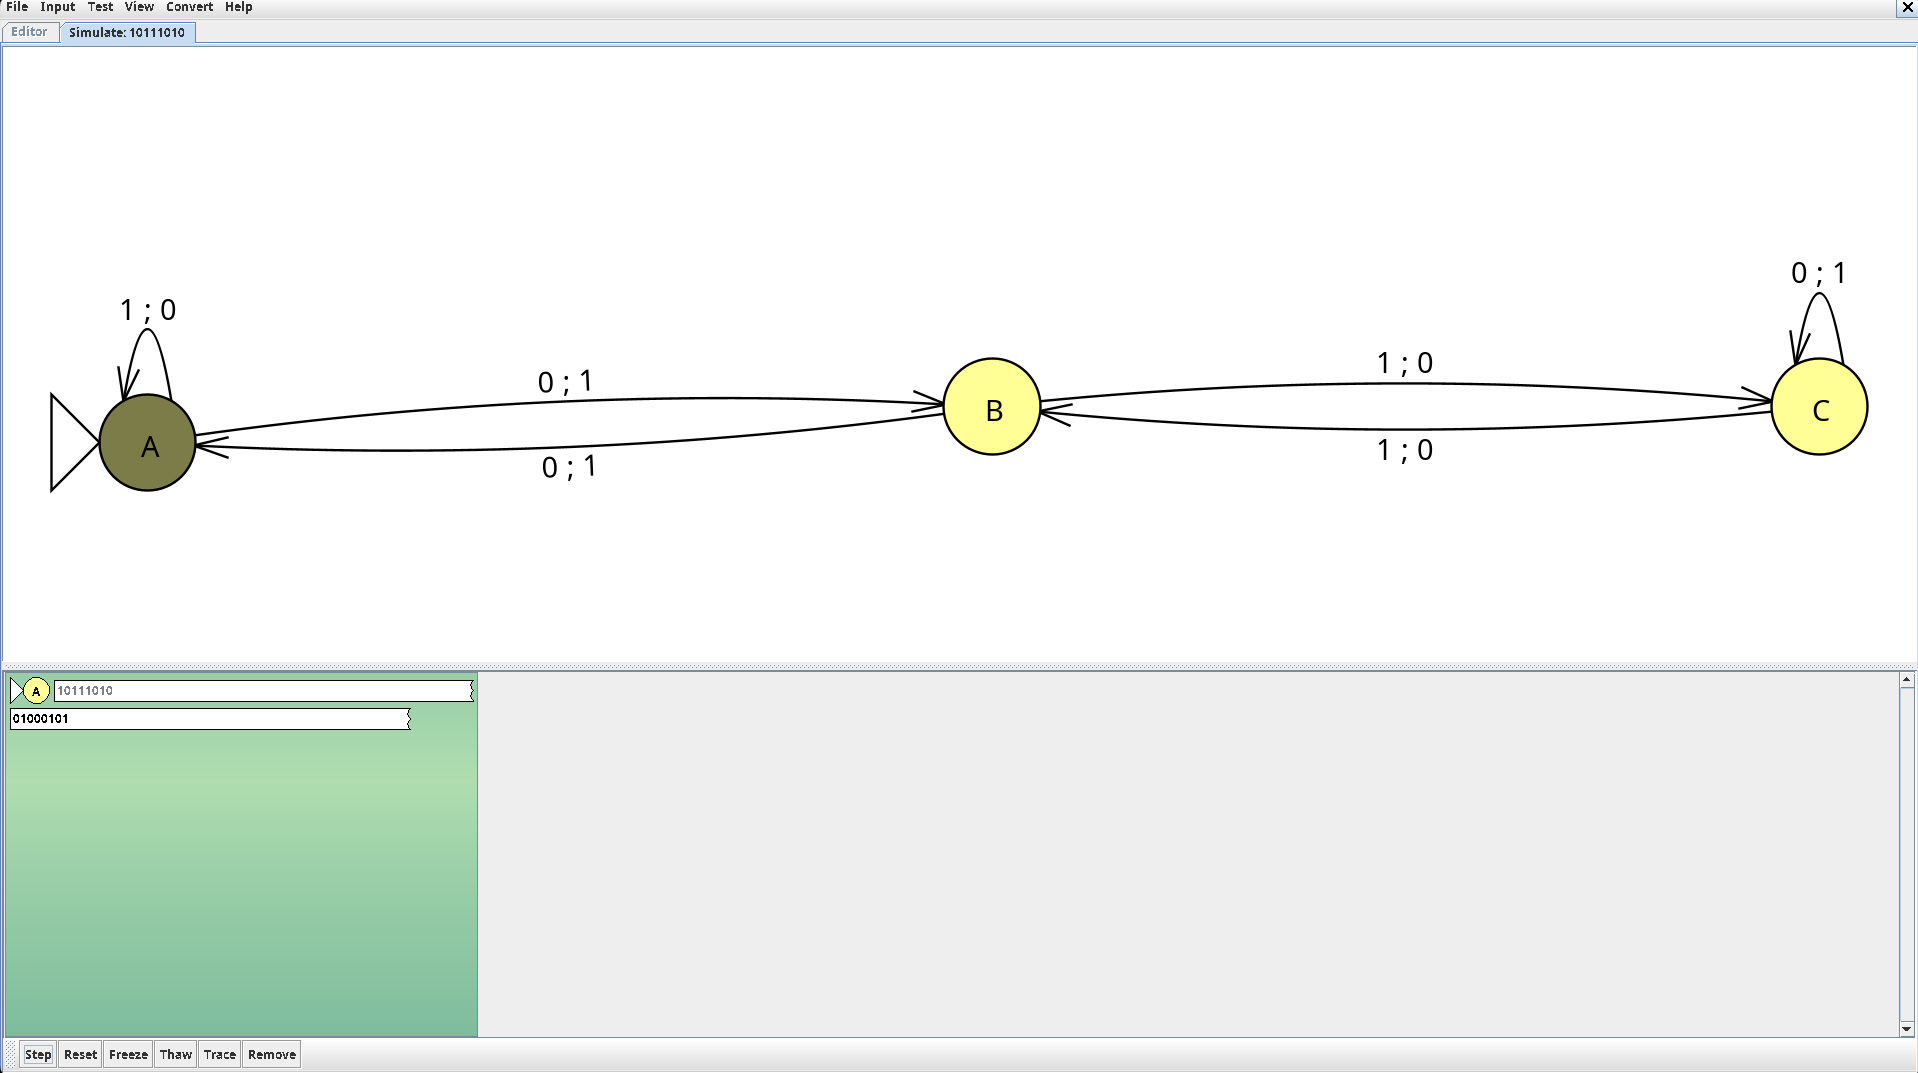
\includegraphics[width=1\textwidth]{./Imagenes/decodificador.png}
        \caption*{(c) decodificador}
    \end{figure}

    \end{document}
